
\documentclass{article}
\usepackage{nips13submit_e,times}

% removed below because it was for IEEE
%\documentclass[letterpaper, 10 pt, conference]{ieeeconf}  % Comment this line out if you need a4paper

% not using IEEE stuff
%\IEEEoverridecommandlockouts                              % This command is only needed if 
                                                          % you want to use the \thanks command
% remove ieee margins
%\overrideIEEEmargins                                      % Needed to meet printer requirements.


%             \documentclass{article}
%             \usepackage{nips13submit_e,times}



\usepackage{prg-stuff}

%\usepackage{ijcai09}  % style
\usepackage{times}    % font
\usepackage{graphicx} % inserting images
\usepackage{cite}
%\usepackage{amsmath}
\usepackage{mathtools} % For math
\usepackage{hyperref}
%\usepackage{enumitem}
\renewcommand{\deg}{\ensuremath{^{\circ}}\xspace}  % why doesn't this work???

\providecommand{\e}[1]{\ensuremath{\times 10^{#1}}}

\graphicspath{ {./figures/} } % Point to the figures directory

%%%%%%%%%%%%%%%%%%%%%%%%%%%%%%%%%%%%%%%%%%%%%%%%%%%%%%%%%%%%%%%%%%%%%%%%%%%

\title{\LARGE \bf 
3D Point Cloud Object Classifier for ROS
}

\author{
Kory E. Kraft\\
School of Mechanical, Industrial, and Manufacturing Engineering,\\
Oregon State University\\
Corvallis, OR, 97330\\
\texttt{kraftko@onid.oregonstate.edu} \\
\And
Austin L. Nicolai\\
School of Mechanical, Industrial, and Manufacturing Engineering,\\
Oregon State University\\
Corvallis, OR, 97330\\
\texttt{nicolaia@onid.oregonstate.edu} \\
}

\newcommand{\fix}{\marginpar{FIX}}
\newcommand{\new}{\marginpar{NEW}}

\nipsfinalcopy 

\begin{document}

\maketitle
\thispagestyle{empty}
\pagestyle{empty}
\begin{abstract}
Many challenging robotics tasks require the ability to manipulate the local environment to complete a
task. Often, due to the difficulty, these tasks are accomplished using shared autonomy or teleoperation.
The need exists for robots to be able to automatically identify and manipulate the local environment on
their own for use in a shared autonomy situation. We implemented a prototype object classifier module for ROS. 
We then classifed four common manipulatives found in many homes as a proof of concept.  
\end{abstract}


\section{Introduction}
Robotics is experiencing an upsurge in research, industry, and popular culture due to 
recent advances in basic robotic abilities.  Driverless vehicles are on the road, and seem to be, in more ways than 
one, right around the corner. However, even with advances in software architecture,
computing hardware, and mechanical hardware, there is still a large gap between what popular culture
 envisions robots doing and what robots can actually do today.

Similarly to computers, there exist tasks that robots can do better than humans, and tasks that humans can do
better than robots. While the ideal is to have fully autonomous robots operating in the world without the need for human intervention, 
there are numerous obstacles preventing that from being the current reality. In order to deploy robots in the real world as quickly as possible, to the benefit of humans, shared autonomy must be exploited to the fullest extent. Finding ways to leverage the strengths of both parties will lead to accelerations in both robot deployment and ability.

Simplifying and streamlining the human-robot interface while using what is readily available in current hardware and software will lead to a better, more fluid shared autonomy experience in less time. Robots are built to interact with the physical world at a level beyond most computer systems. To this end, they must sense the environment in order to interact with it. The Microsoft Kinect RGB-D camera is a low-cost solution for many computer vision tasks required of a robot. On the software side, the Robot Operating System (ROS), is a software system and set of libraries that currently handles basic information processing for robots in a hardware-independent manner.

What is missing between the two is a simple framework with a clean interface that unites the current hardware and software capabilities for the purposes of object classification that will then be used for object manipulation during a shared autonomy session. To this end, we built a prototype program that utilized ROS-formatted data streams from a Microsoft Kinect along with the PyBrain machine learning package to classify four common manipulative objects: a door knob, a light switch, a drawer handle, and a shower knob. These objects were classified using 3D point cloud information obtained via a Kinect sensor. Having a streamlined data-to-classification program will improve the current state of the art shared autonomy approach for object manipulation by removing a previously time-consuming step on the part of the human user.

\section{Related Work}
\subsection{Shared Autonomy}
\begin{figure}[h!]
    \centering
    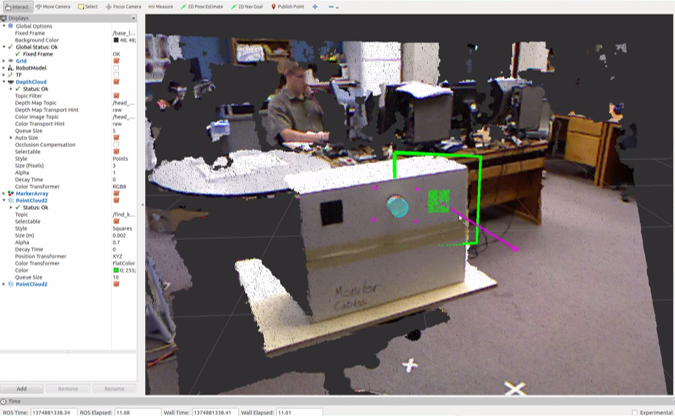
\includegraphics[width=0.45\textwidth]{Shared_Autonomy_1.png}
    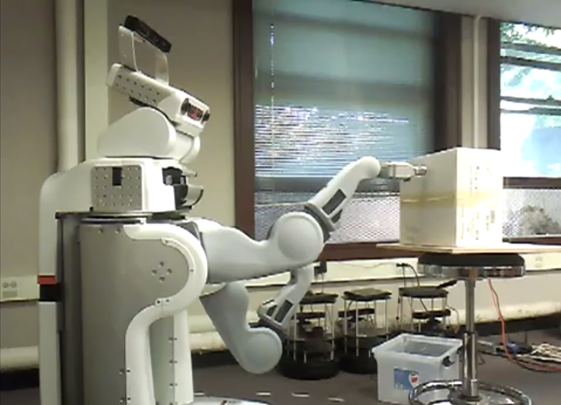
\includegraphics[width=0.45\textwidth]{Shared_Autonomy_2.png}
    \caption{Right: The user-interface for a shared autonomy session. Left: PR2 manipulates a shower knob in a teleoperation session using MoveIt!.}
    \label{fig:sharedAutonomy}
\end{figure}

In the world of robots, there is a spectrum of autonomous function.  On one end, there is a fully autonomous robot
without the need for human intervention in the direction of basic tasks.  Think, driverless vehicles that only need to be told a destination, and then the rest is done automatically.  On the other end is remote teleoperation that requires a human expert to constantly inform and direct the robot.  Think, a scientist sitting at a desktop using a joystick to control all the movements of a research submersible. Shared autonomy lies in the middle between these two extremes \cite{sharedAutonomy}. 

Shared autonomy requires that a robot be able to do some things on its own (e.g. raise its gripper hand or drive forward), while allowing
 a human in the loop to direct or give meaning to the robot's actions. Work has been done to create an interface that
allows a human operator to give overall guidance to the robot in terms of where to go. The human operator must then identify the general region of the manipulative object in a GUI via a drag-and-drop action sequence.  The object is identified by having the operator ``paint'' the object in the GUI with the mouse.  Finally, a checkbox is used to classify the object.  Only after this can the robot manipulate the selected controller (Figure \ref{fig:sharedAutonomy})\cite{matt}. 

We want to simplify this process by having the robot classify the object once the general regoin of the object is selected by the user, thus further autonomizing the robot's actions.

\subsection{Object Classification}
Automatic classification of images and objects has long been an important task in machine learning. With the proliferation of lower cost depth capable sensors (e.g. the Microsoft Kinect) more work is being done classifying point cloud data.

Specifically, object detection and classification using the Microsoft Kinect has been widely examined. Janoch, et al. present a large 3D dataset comprised of over 50 classes after determining that many current 3D datasets are lacking in scene and category variation. They further provide a method to smooth the noisy depth data provided by the Kinect, and establish baseline object detection rates \cite{kinectWork}. Another application by Greuter, et al. uses Kinect point cloud data to detect game pieces (specifically, chess) and determine their board location \cite{eurobot}. They were able to achieve an approximate 84\% success rate.

In the realm of personal robotics, Rusu, et al. examine the use of 3D point cloud based mapping and recognition in household environments. They present a method in which an environment is mapped once, then in real-time, 3D point cloud data obtained by the laser scans is correlated to the known scene. The data is then segmented into regions, allowing kitchen objects to be identified (e.g. a cupboard, drawer, dishwasher, etc). Through real world testing, they were able to experimentally validate their results \cite{mapKitchen, mapHouse}. 

\subsection{ROS}
The Robot Operating System (ROS), which has its deepest roots in the Stanford AI group and former Willow Garage, 
has become the leader in open-source robotics software \cite{ros, rospaper}. ROS is written largely in C++ and Python (termed rospy) and runs on top of Ubuntu.  

It is used by hobbyists, researchers, and major industrial manufacturers, and has a large pool of active developers. The software library is vast, and due to the hardware agnostic nature of the system, ROS can run on many different robot platforms.  ROS includes tools for basic robot sensing, movement, and simulators that allow programmers to test code before deploying it on a physical robot. Although ROS is guided by Open Source Robotics Foundation (OSRF), ROS relies on the larger community to maintain and extend its capabilities \cite{ros, OSRF}.

ROS includes packages for teleoperation, using the keyboard and mouse, or even operating the robot utilizing a Razer Hydra controller and Oculus Rift headset \cite{surrogate}. ROS also includes MoveIt!, a path-planning and object manipulation software \cite{moveit}. 

Given all of the benefits of ROS, we were somewhat surprised to find that there was not a streamlined, one-step program and interface to allow users to gather data, train, and classify sets of objects based on 3D point cloud information.  This could then be used in conjunction with the shared autonomy approach and MoveIt! described above.

\subsection{Microsoft Kinect}
The Microsoft Kinect was introduced to the marketplace in 2010 \cite{kinectHistory}. Since then 
it has found its way into research labs as well as living rooms.
It provides RGB-D sensing for less than 100 dollars. It has become a standard RGB-D
sensing device due to its low price point, extensive documentation, and large community of
adopters. The original Kinect is limited to 0.8 - 4.0m distance range and 57$^{\circ}$ horizontal 
and 43$^{\circ}$ vertical field-of-view. 

The device is not flawless; it has a random error in the depth axis 
ranging from a few mm to 4 cm in a non-uniform distribution \cite{khoshelham2012accuracy,nguyen2012modeling}.
Kinect v2 has been released that provides 3x better depth fidelity and improved small object visualization compared to 
the original Kinect \cite{kinect}. We used the original Kinect for our project that will provide a baseline for manipulative classification, knowing
it will only be improved upon in the future.

\subsection{PyBrain}
PyBrain describes itself as ``a modular Machine Learning Library for Python.'' The open-source module focuses on neural networks and offers ways to quickly build and train neural networks, even for beginning programmers. PyBrain includes Python bindings to use other popular products like LibSvm \cite{pybrain, pybrainCode}.  

PyBrain works well alongside ROS, and depends heavily upon SciPy which is included with rospy.

\section{Methods}
\subsection{Objects}
\begin{figure}[h!]
    \centering
    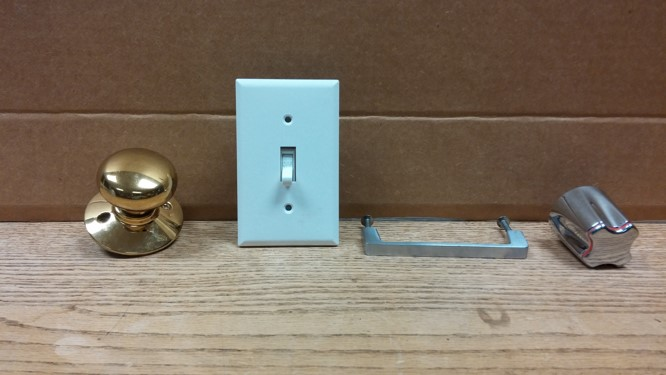
\includegraphics[width=0.45\textwidth]{All_Knobs.jpg}
    \caption{Objects Classified: door knob, light switch, drawer handle, shower knob}
    \label{fig:objects}
\end{figure}
We decided to classify four common household objects: a door knob, light switch, drawer handle, shower knob. These objects were selected
for their ubiquity in many residences and living environments. See Figure \ref{fig:objects}.

\subsection{Data Capture}

We chose to capture the data in such a way that can be easily adapted to a near-future operation environment in which a robot will be instructed via a human trainer to ``learn'' an image that the human is pointing to.  Only capturing 5 seconds of data ensures that the capture time will be more seamless, and will not result in the human trainer waiting for enormous amounts of time for the robot to ``take in'' the scene.  
% possibly good location for 2 figs.
We captured data utilizing the Microsoft Kinect and subscribing to the related ROS topic.  The data was recorded in the standard ROS format, rosbag.  Even though we did this via a stationary laptop, we were running a virtual instance of ROS to issue the commands. This means that any robot running ROS has access to the same commands and data format. 

For ease of operability, and to have standardized image distances during the first iteration, the Kinect  was detached from a robot and placed on a tripod, with the manipulative object in the middle of the Kinect's field-of-view. We kept the Kinect at the same height and distance (0.8 m) while capturing the data. Approximately 5 seconds of data were captured for each manipulative (and blank backdrop) at each viewing angle. The three viewing angles, in terms of the horizontal viewing axis, were: 90, with \(\pm\)20$^{\circ}$ variations.

The Kinect sensor provides both point cloud and RGB data at resolution of 640 x 480. For every one second of recording, approximately 10 RGB point clouds were stored.

\subsection{Data Parsing}

\begin{figure}
	\centering
	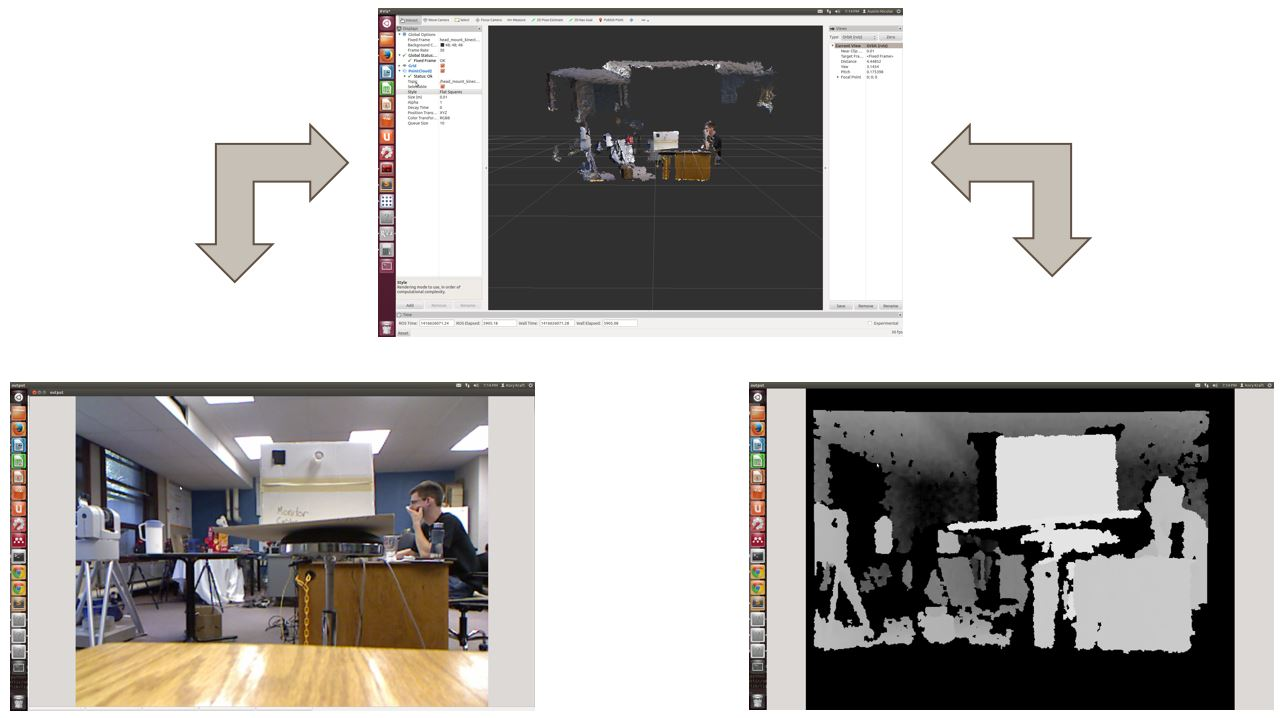
\includegraphics[width=1.0\textwidth]{RVIZ_Decomposition.JPG}
	\caption{Kinect point cloud data decomposed into RGB and depth data}
	\label{fig:RVIZ_decomp}
\end{figure}
\begin{figure*}
    \centering
    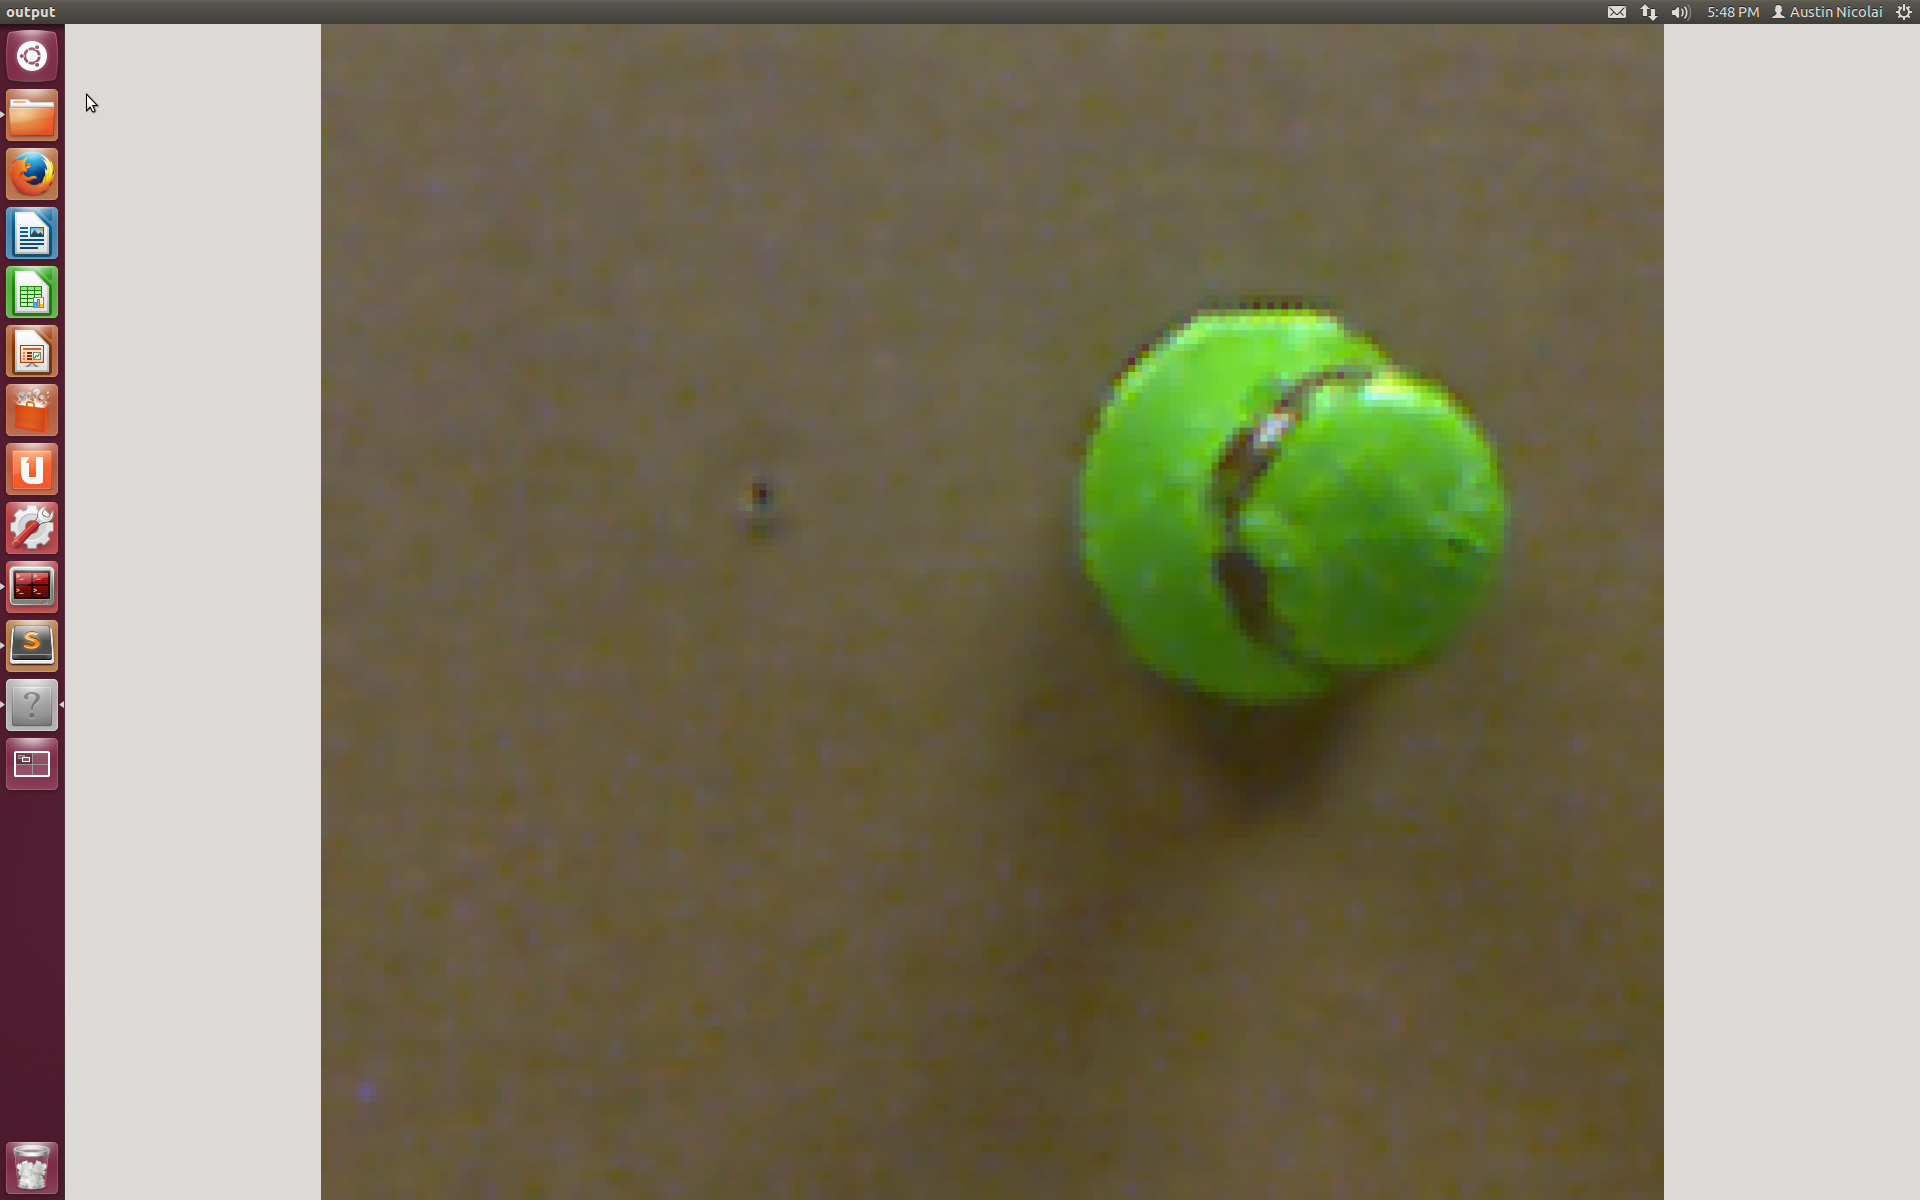
\includegraphics[width=0.3\textwidth]{DH_RGB_L.png}
    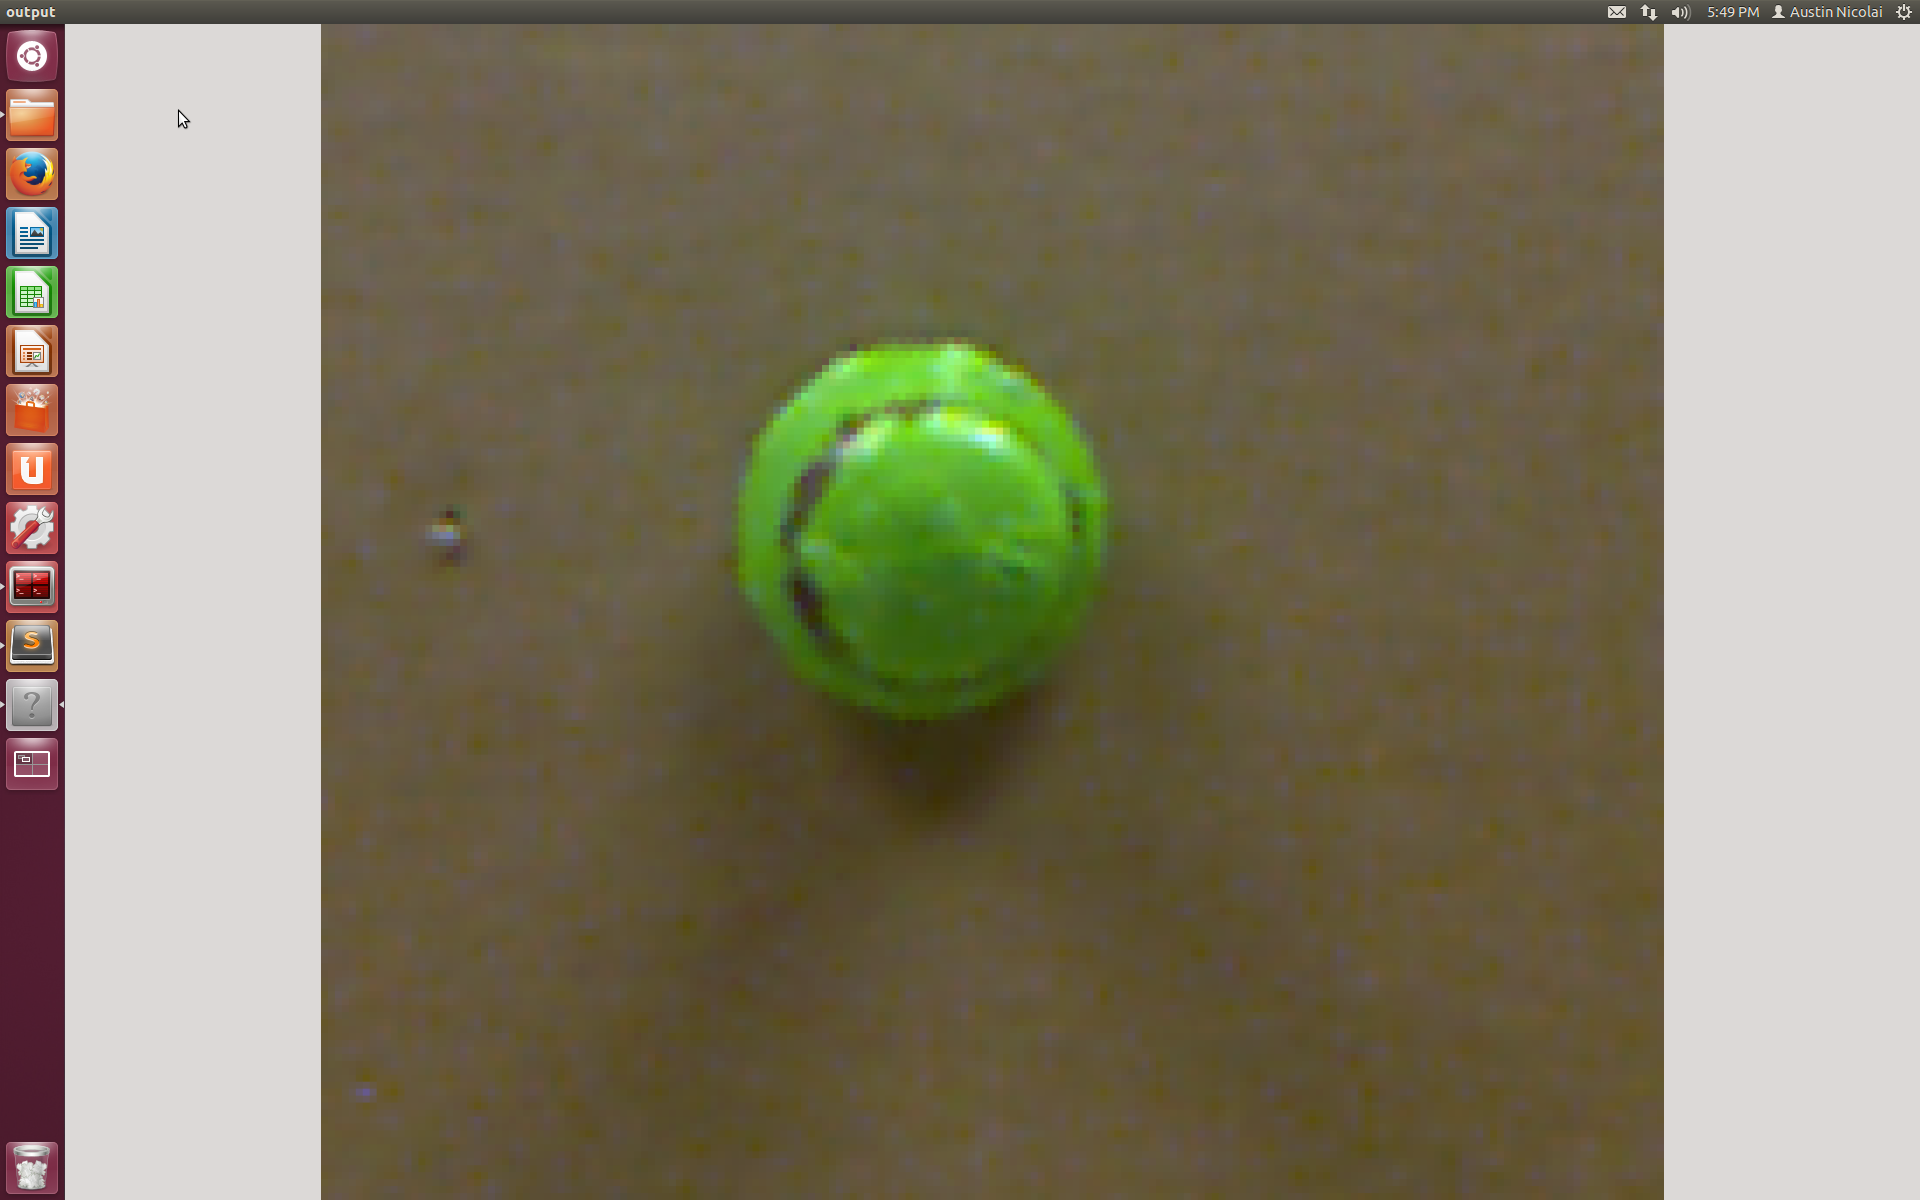
\includegraphics[width=0.3\textwidth]{DH_RGB_C.png}
    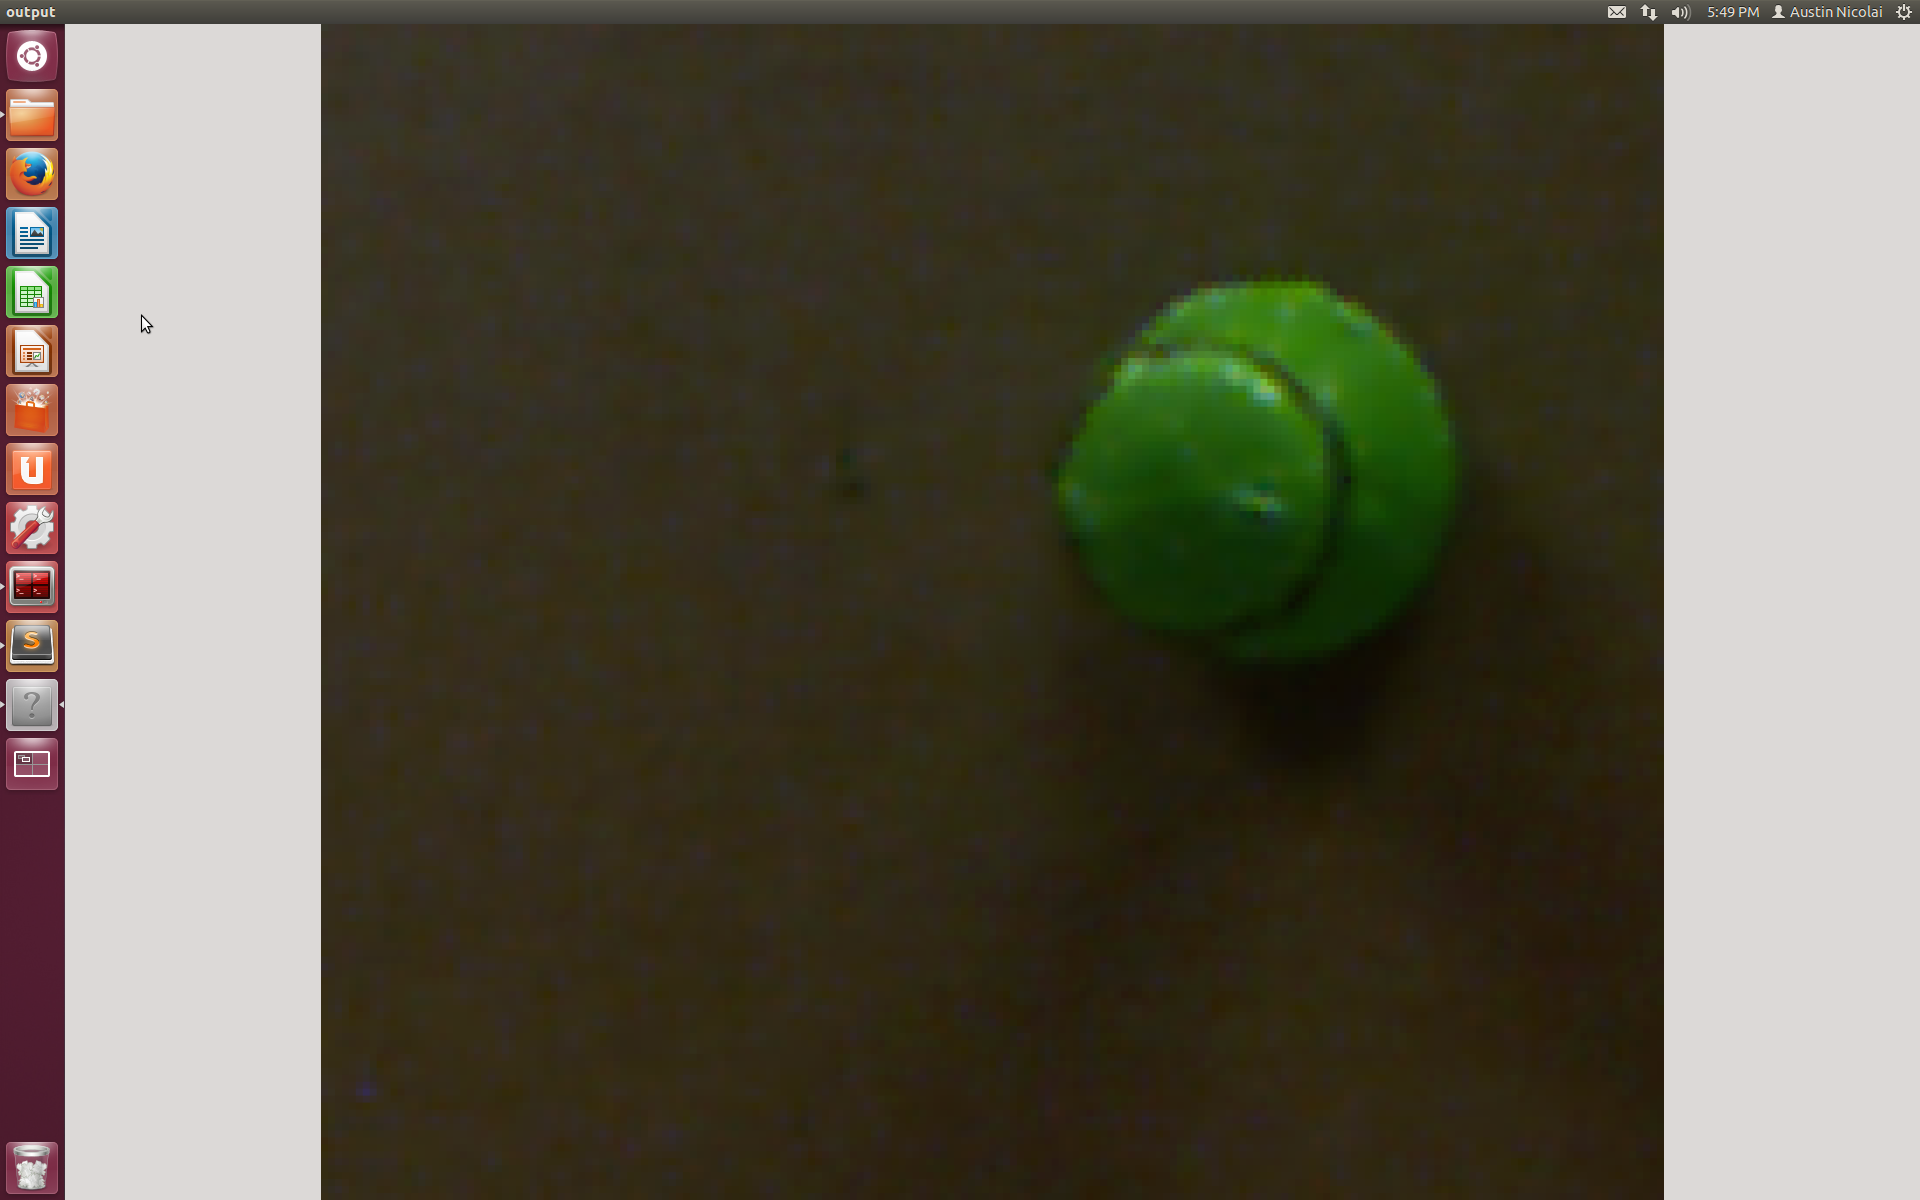
\includegraphics[width=0.3\textwidth]{DH_RGB_R.png}
    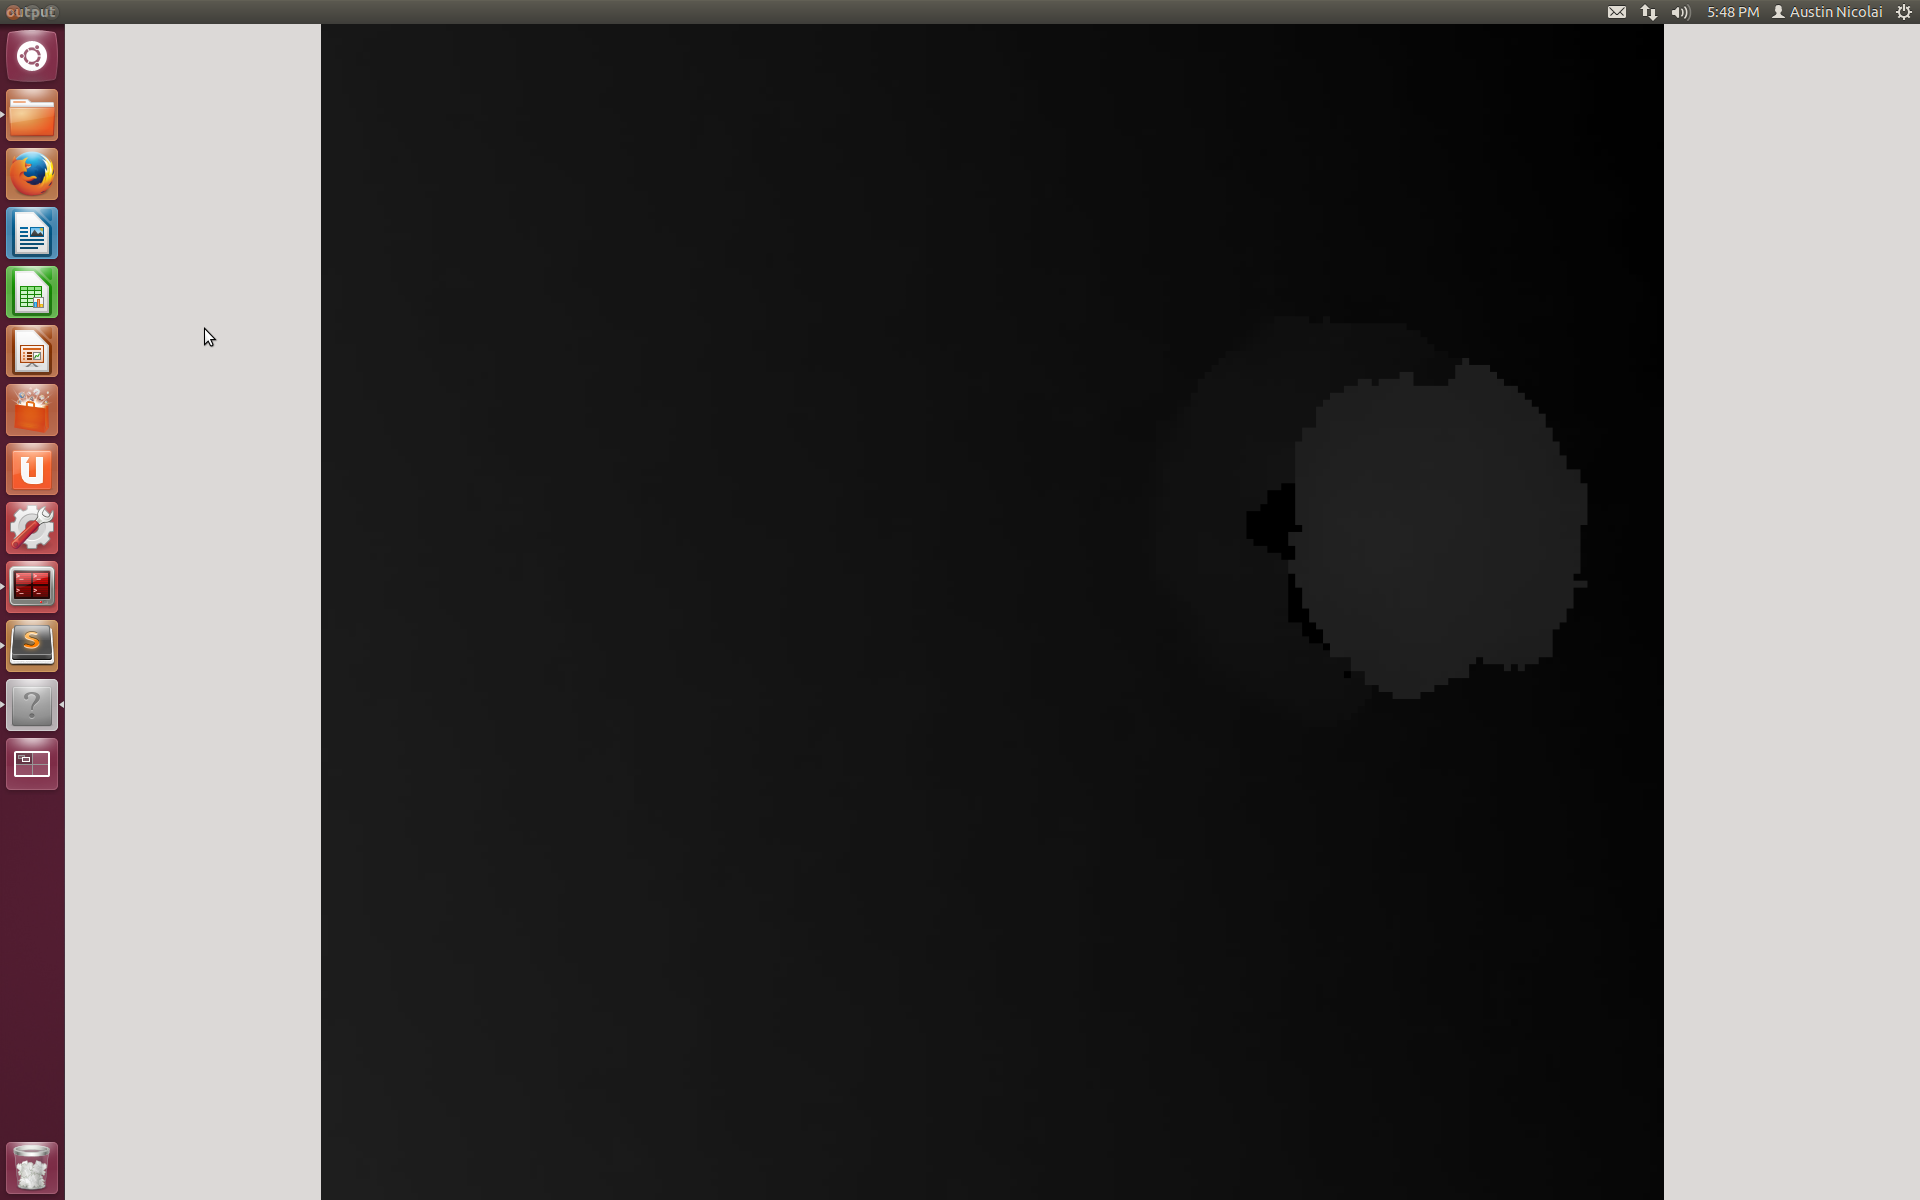
\includegraphics[width=0.3\textwidth]{DH_D_L.png}
    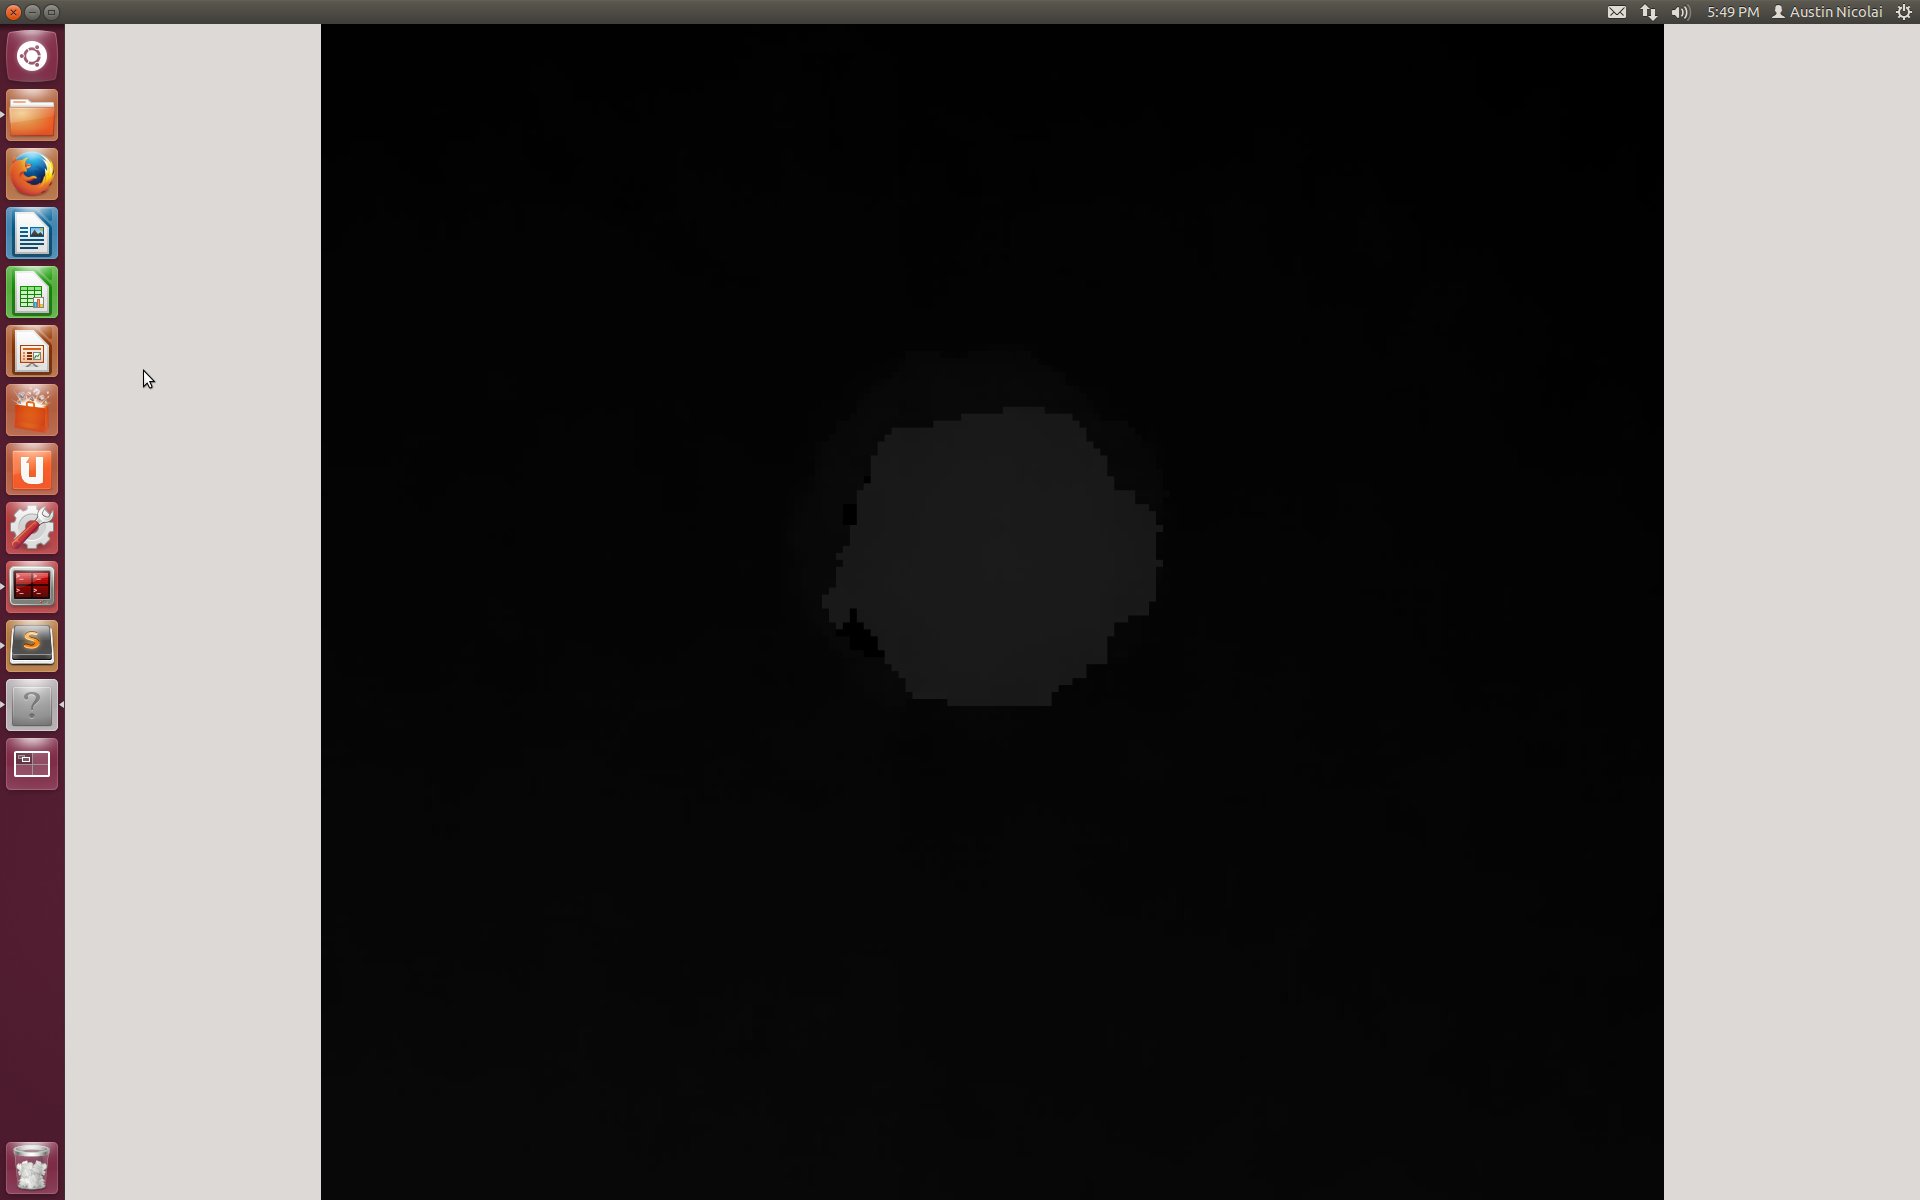
\includegraphics[width=0.3\textwidth]{DH_D_C.png}
    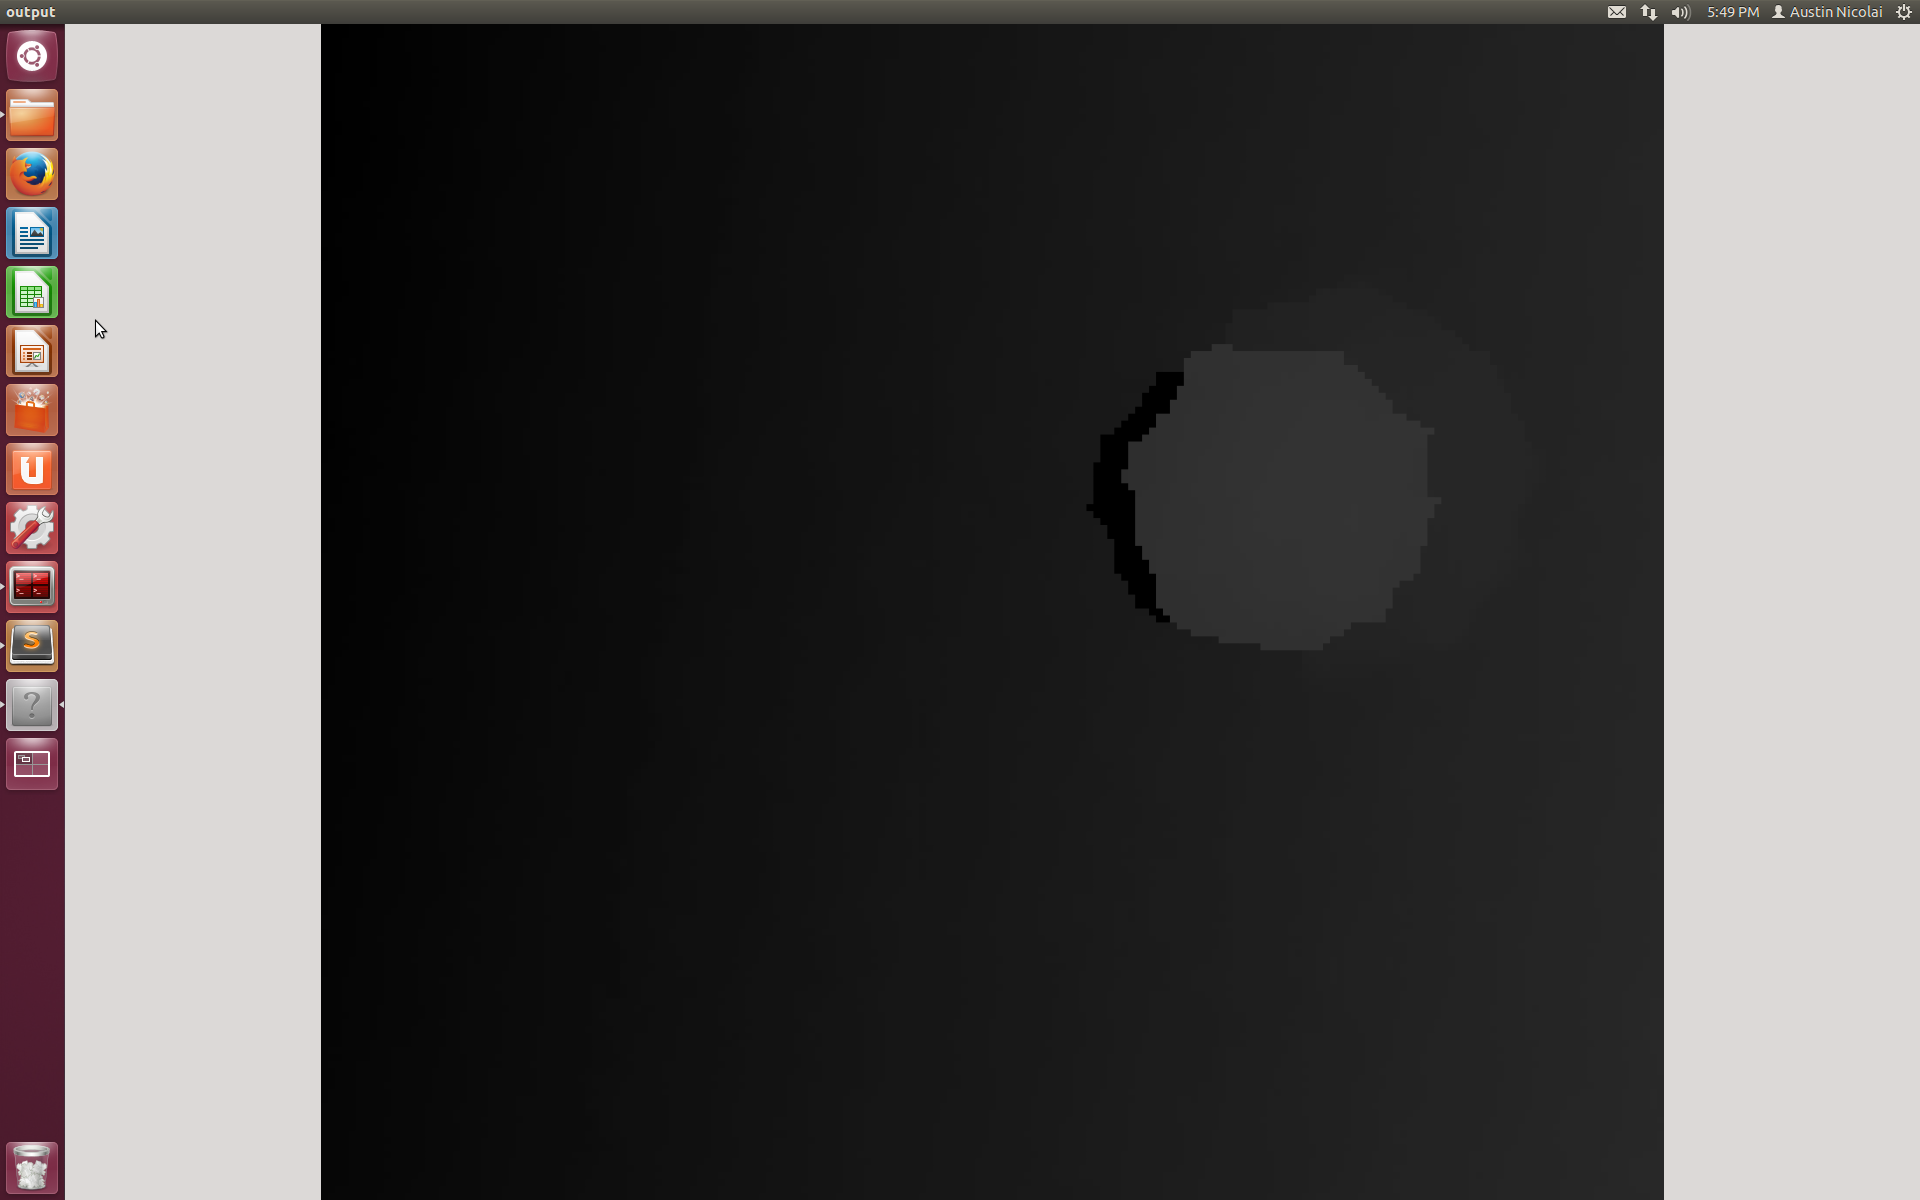
\includegraphics[width=0.3\textwidth]{DH_D_R.png}
    \caption{Door knob data decomposed into the RGB and normalized greyscale depth values as viewed from the left, center and right.}
    \label{fig:decomposition}
    
\end{figure*}
We decomposed the captured RGB point cloud in Python utilizing self-written code and ros-pcl, a ROS interface to the open-source Point Cloud Library (PCL)\cite{pcl, rospcl}. The point cloud data was then decomposed into a 640 x 480 RGB image and a 640 x 480 depth image (see Figure \ref{fig:RVIZ_decomp}). The depth image was represented in greyscale, with intensity values normalized to the range 0 - 255. See Figure \ref{fig:decomposition} for an example of the different view angles, decomposed, for the door knob object.

Only the depth values were considered for inputs to the neural network. In order to reduce the number of inputs to the neural network, the 640 x 480 depth image was cropped to the center 30\% of the pixels. This resulted in an input image sized 192 x 144. This 2D matrix was further converted into a single row vector for input to the neural network.

\subsection{Learning}
The data was randomly split into 80\% training data and 20\% testing data. The neural network consisted of 27,648 inputs, one for each value in the normalized, cropped depth matrix.  There were 25 hidden neurons and 5 outputs. Each output represented the class labels for the 4 knobs plus the blank backdrop. The predicted classification label was taken to be the largest value of the outputs. The neural network was trained using backpropagation for 1000 epochs. Training time lasted approximately 6 hours.

\section{Results}
\begin{figure}[!b]
    \centering
    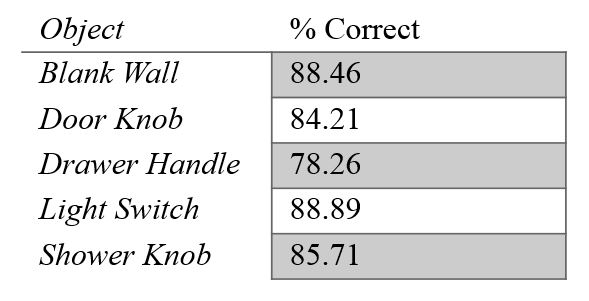
\includegraphics[width=0.5\textwidth]{Results_1.JPG}
    \caption{Object identification rate, per object, for test samples}
    \label{fig:results1}
\end{figure}
\begin{figure}[!t]
    \centering
    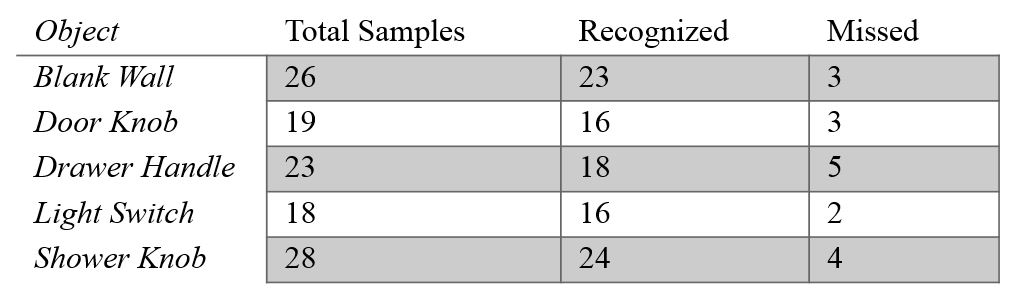
\includegraphics[width=0.9\textwidth]{Results_2.JPG}
    \caption{Object classification tally for test samples}
    \label{fig:results2}
\end{figure}
\begin{figure}[!t]
    \centering
    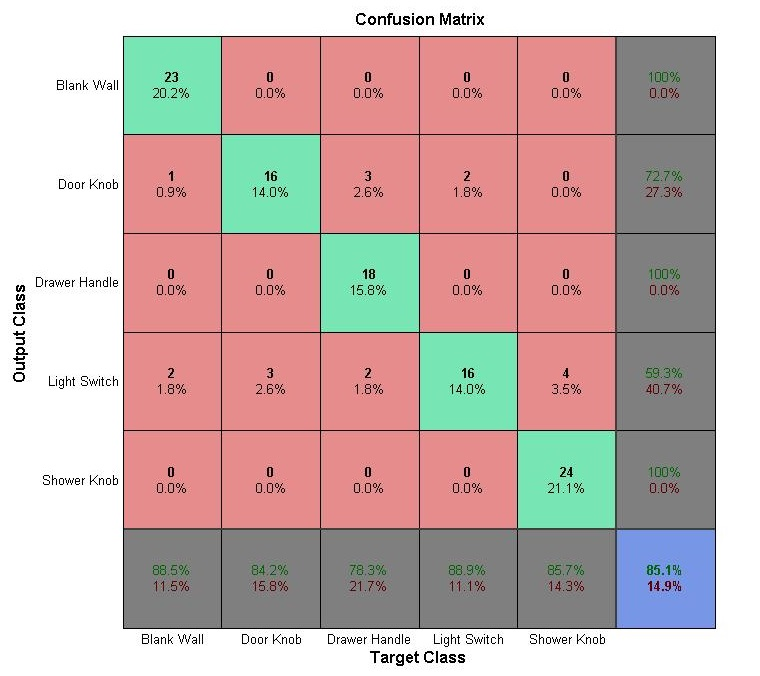
\includegraphics[width=.8\textwidth]{confusion.jpg}
    \caption{Confusion matrix}
    \label{fig:confusion}
\end{figure}

Overall, the classification success rate for the four objects was high, much greater than random (see Figures \ref{fig:results1} and \ref{fig:results2}). While all objects had a roughly 80\% - 90\% successful classification rate, more insight into the system can be gained from understanding how the misclassifications occurred.

As can be seen in Figure \ref{fig:confusion}, if a knob was misclassified, it was often misclassified as a light switch. This can potentially be explained, in part, by the Kinect sensor noise. In addition, occasionally the Kinect is unable to return depth data of any sort for specific regions of the image (due to surface reflections, etc). In these cases, the neural network may only be provided with a small amount of meaningful depth information for the manipulatable object. To the neural network, this likely appears to approximate the light switch object. This is because the light switch object itself appears to be a nearly flat wall, with a small area of changing depth information (the actual switch).

Even though the training time on the neural network was longer than we hoped, it was of such duration that the robot could ``train'' on a new set of objects while a person was away at work, at home sleeping, or absorbed in another task.

\newpage

\section{Future Work}
The analysis of our results presents several opportunities for further research.

First off, the module we designed needs to be packaged up, with accompanying documentation, and deployed for other ROS users. The module could be further extended to allow users to select which type of classification method (e.g. SVM, neural network, etc.) they would like to use. Similarly, the module could be extended to 
allow for users to utilize PCA or other feature reduction methods, if so desired.

Lastly, the module could be deployed and tied in with the shared autonomy approach mentioned above. Once done, the overall action sequence could be 
tested to see how much speed-up is gained when trying to manipulate an object using the new shared autonomy action sequence.

\bibliographystyle{IEEEtran}
\bibliography{main}


\end{document}
